\documentclass[a4paper]{article}
\usepackage[utf8]{inputenc}
\usepackage{alphabeta}
\usepackage{graphicx}
\usepackage[section]{placeins}
\usepackage{float}
\usepackage{amsmath}
\usepackage{listings}
\usepackage{xcolor}
\usepackage{amsmath}
\usepackage{extarrows}
\usepackage{amssymb}

\definecolor{codegreen}{rgb}{0,0.6,0}
\definecolor{codegray}{rgb}{0.5,0.5,0.5}
\definecolor{codepurple}{rgb}{0.58,0,0.82}
\definecolor{backcolour}{rgb}{0.95,0.95,0.92}

\lstdefinestyle{mystyle}{
    backgroundcolor=\color{backcolour},   
    commentstyle=\color{codegreen},
    keywordstyle=\color{magenta},
    numberstyle=\tiny\color{codegray},
    stringstyle=\color{codepurple},
    basicstyle=\ttfamily\footnotesize,
    breakatwhitespace=false,         
    breaklines=true,                 
    captionpos=b,                    
    keepspaces=true,                 
    numbers=left,                    
    numbersep=5pt,                  
    showspaces=false,                
    showstringspaces=false,
    showtabs=false,                  
    tabsize=2
}

\lstset{style=mystyle}

\setlength{\parindent}{0pt}
\setlength{\parskip}{1em}
\setlength{\jot}{4mm}

\title{Συστήματα Αναμονής, 1η εργαστηριακή άσκηση}
\author{Νικόλαος Παγώνας, el18175}
\date{Απρίλιος 2021}

\begin{document}

\maketitle

\section*{Κατανομή Poisson} 

\subsection*{Α.}

Με τη βοήθεια του πακέτου \textbf{statistics} της Octave και της συνάρτησης \textbf{stem}, απεικονίζουμε τη συνάρτηση μάζας πιθανότητας της κατανομής Poisson, για $ {λ = \{3,10,50\}} $.

\begin{figure}[H]
	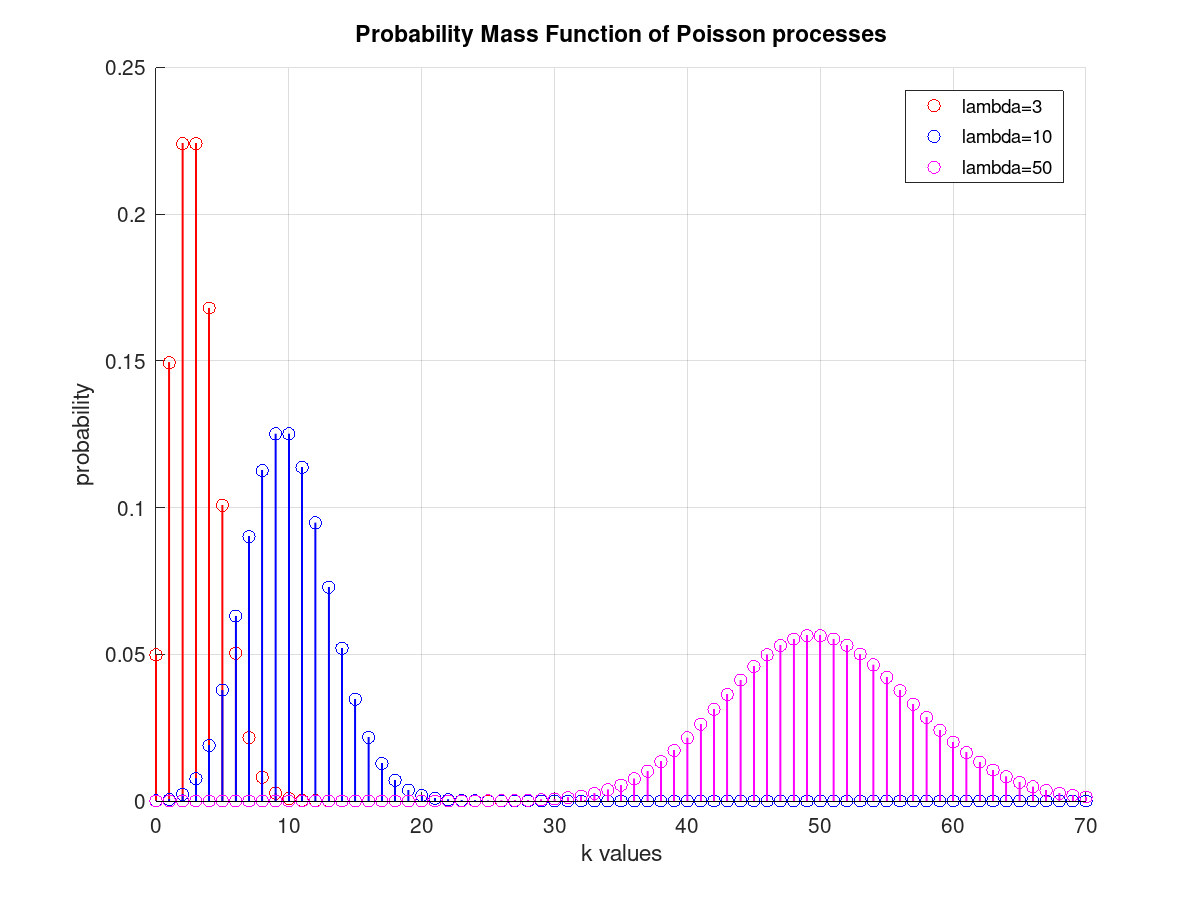
\includegraphics[width=\textwidth]{../images/Poisson_Distribution_A.png}
	\caption{Probability Mass Function of Poisson processes}
	\label{fig:Poisson Distribution A}
\end{figure}


Παρατηρούμε ότι όσο μεγαλώνει η τιμή της παραμέτρου $ λ $:
\begin{enumerate}	
	\item η κατανομή ``απλώνεται'', δηλαδή οι τιμές των θέσεων αριστερά και δεξιά από την μέση τιμή της κατανομής αυξάνονται. Αυτό είναι λογικό, αφού η διακύμανσή της, που είναι ίση με $ λ $, αυξάνεται. 
	\item η θέση όπου η κατανομή είναι μέγιστη, πηγαίνει προς τα δεξιά. Αυτό συμβαίνει γιατί η μέση τιμή της (επίσης ίση με $ λ $) αυξάνεται.
	\item η μέγιστη τιμή της κατανομής μειώνεται. Αυτό συμβαίνει γιατί πρέπει να ικανοποιείται η ιδιότητα:
	\[
		\sum_{x} P(X = x) = 1,
	\]
	η οποία ισχύει για κάθε διακριτή τυχαία μεταβλητή. Έτσι, αφού οι τιμές αριστερά και δεξιά της μέσης τιμής αυξάνονται, το μέγιστο οφείλει να μειωθεί και η κατανομή ``χαμηλώνει'' συνολικά. 
\end{enumerate}

\subsection*{Β.}

Με βάση τους ορισμούς της μέσης τιμής και της διακύμανσης:

\[
	E[X]=\sum_x x P(X=x)
\]
και 
\[
	Var[X] = Ε[X^2]-Ε^2[X]
\]

Έτσι, για $ λ = 30 $ έχουμε:

\lstinputlisting{../images/Poisson_Distribution_B.txt}

Οπότε επαληθεύουμε και μέσω της προσομοίωσης αυτό που ξέρουμε ότι ισχύει από τη θεωρία για την κατανομή Poisson: 

\[ 
	{Ε[X] = Var[X] = λ = 30} 
\]


\subsection*{Γ.}

Επιλέγουμε τις κατανομές Poisson με παραμέτρους $ λ = 10 $ και $ λ = 50 $. Γνωρίζουμε από τη Θεωρία Πιθανοτήτων ότι η κατανομή της τυχαίας μεταβλητής $ {Z = X + Y} $ προκύπτει από την συνέλιξη των κατανομών των X και Y (εδώ κάνουμε την υπόθεση ότι οι X και Y είναι ανεξάρτητες). 

Απεικονίζουμε τις κατανομές των $ X\sim Pois(10), Y \sim Pois(50) $ και $ {Z = X + Y }$:

\begin{figure}[H]
	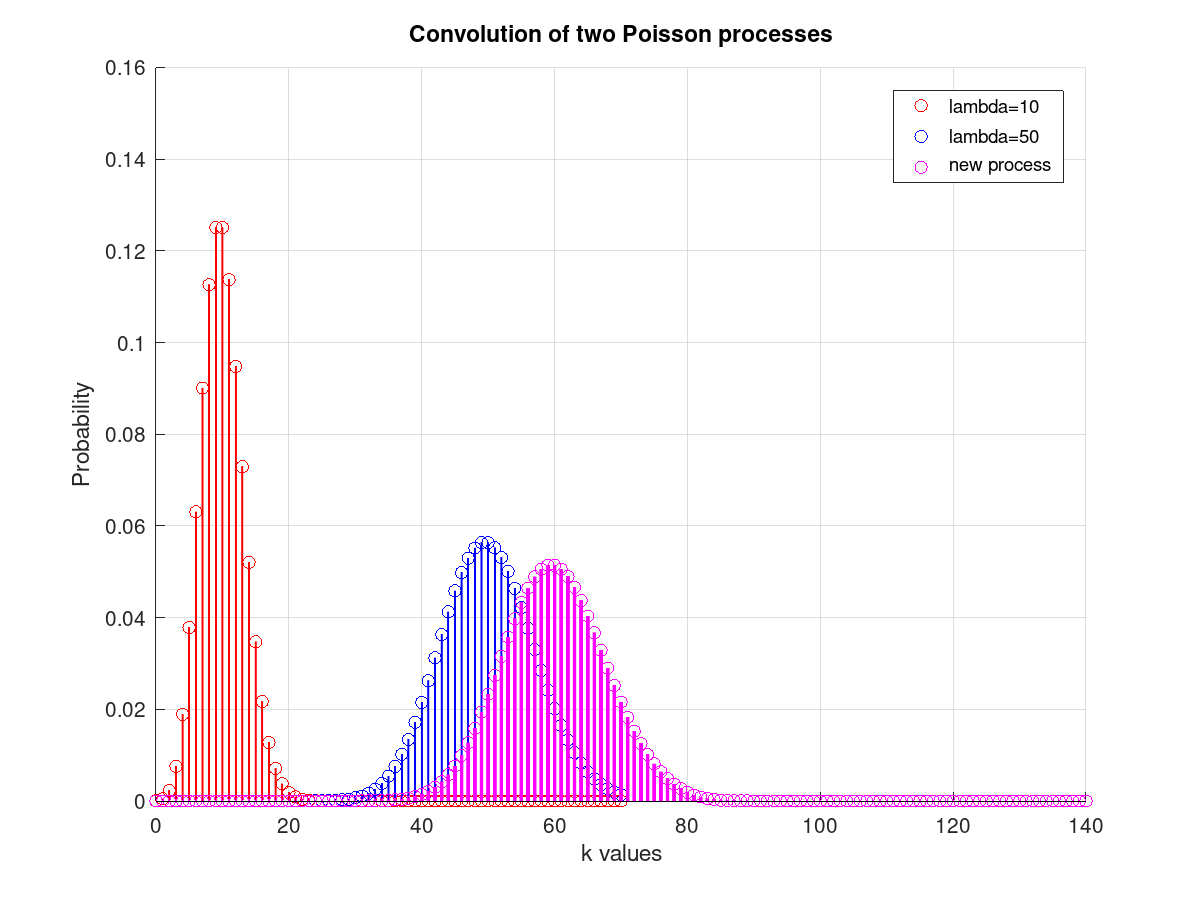
\includegraphics[width=\textwidth]{../images/Poisson_Distribution_C.png}
	\caption{Convolution of two Poisson processes}
	\label{fig:Poisson Distribution C}
\end{figure}

Παρατηρούμε ότι προκύπτει κατανομή \textbf{Poisson} με μέση τιμή 60. Αυτό είναι λογικό, αφού γνωρίζουμε πως το άθροισμα δύο τυχαίων μεταβλητών Poisson με παραμέτρους $ {λ_1, λ_2} $ ακολουθεί κατανομή Poisson με παράμετρο $ {λ_1 + λ_2} $. Απαραίτητη προϋπόθεση για να ισχύει αυτό είναι οι τυχαίες μεταβλητές να είναι \textbf{ανεξάρτητες}.

\subsection*{Δ.}

Αποδεικνύουμε τον παραπάνω ισχυρισμό:

Έστω ένα διάστημα χρόνου $ t $.

\begin{itemize}
	\item Διαιρούμε το διάστημα $ t $ σε $ n $ υποδιαστήματα, $ {t = nΔt} $
	\item Πραγματοποιούμε $ n $ ανεξάρτητες δοκιμές Bernoulli, μία σε κάθε υποδιάστημα, με πιθανότητα επιτυχίας $ {p = λΔt} $
	\item Έτσι, η πιθανότητα $ k $ επιτυχιών σε $ n $ ανεξάρτητες δοκιμές δίνεται από την Διωνυμική Κατανομή:
	\begin{align*}
		P[N(t) = k] &= \binom{n}{k}p^k(1-p)^{n-k}, \ k = 0,1,...,n \\
						&= \binom{n}{k}(λΔt)^k(1-λΔt)^{n-k} \\
						&= \binom{n}{k}\left(\frac{λt}{n}\right)^k\left(1-\frac{λt}{n} \right)^{n-k} \\			
	\end{align*}
	\item Και για $ Δt \to 0, n \to \infty $, έχουμε 
	\[
		\frac{n!}{(n-k)!} \to n^k, \ \left( 1-\frac{λt}{n}\right)^{n-k} \to e^{-λt},
	\]
	οπότε 
	\[
		P[N(t)=k] = \frac{n!}{k!(n-k)!}\left( \frac{λt}{n}\right)^k \left(1-\frac{λt}{n}\right)^{n-k} \to \frac{(λt)^k}{k!}e^{-λt}. \ \ \ \blacksquare
	\]
\end{itemize} 

Με αυτόν τον τρόπο ($ λ = np $, όπου $ n $ μεγάλο και $ p $ μικρό), μπορούμε να κατασκευάσουμε μία κατανομή Poisson παραμέτρου $ λ = 30 \ \frac{\text{σημεία}}{\text{sec}}$. Επιλέγουμε $ n = 30, 60, 90, 120, 150 $. 

\begin{figure}[H]
	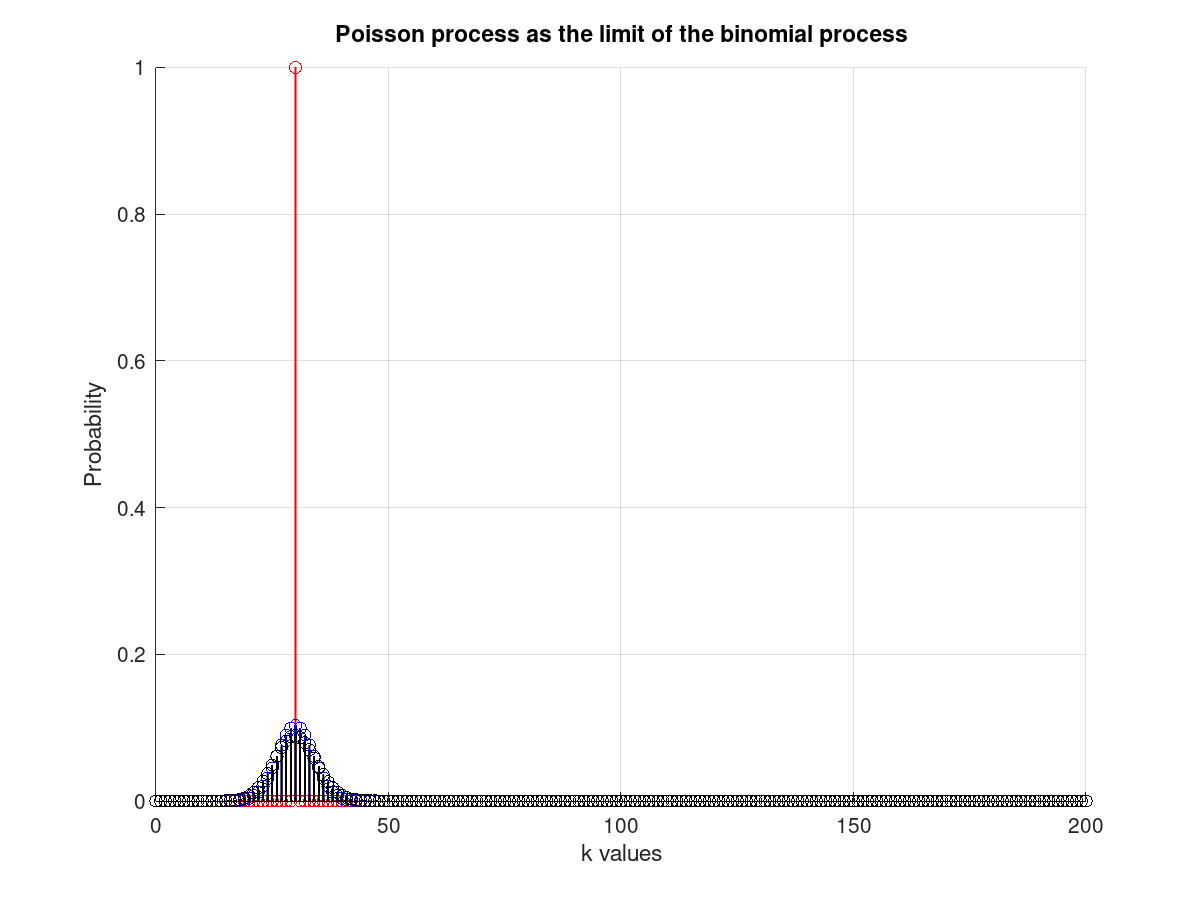
\includegraphics[width=\textwidth]{../images/Poisson_Distribution_D.png}
	\caption{Poisson process as the limit of the binomial process}
	\label{fig:Poisson Distribution D}
\end{figure}

Παρατηρούμε ότι όσο το n αυξάνει, τόσο η διωνυμική κατανομή προσεγγίζει καλύτερα την Poisson.

\section*{Εκθετική Κατανομή}

\subsection*{Α.}

Απεικονίζουμε στο Octave την συνάρτηση πυκνότητας πιθανότητας της εκθετικής κατανομής, με μέσο όρο $\frac{1}{λ}=\{0.5,1,3\}$. Χρησιμοποιώντας πολύ μικρό βήμα (k = 0:0.00001:8) μπορούμε να προσεγγίσουμε με μεγάλη ακρίβεια την συνεχή εκθετική κατανομή:

\begin{figure}[H]
	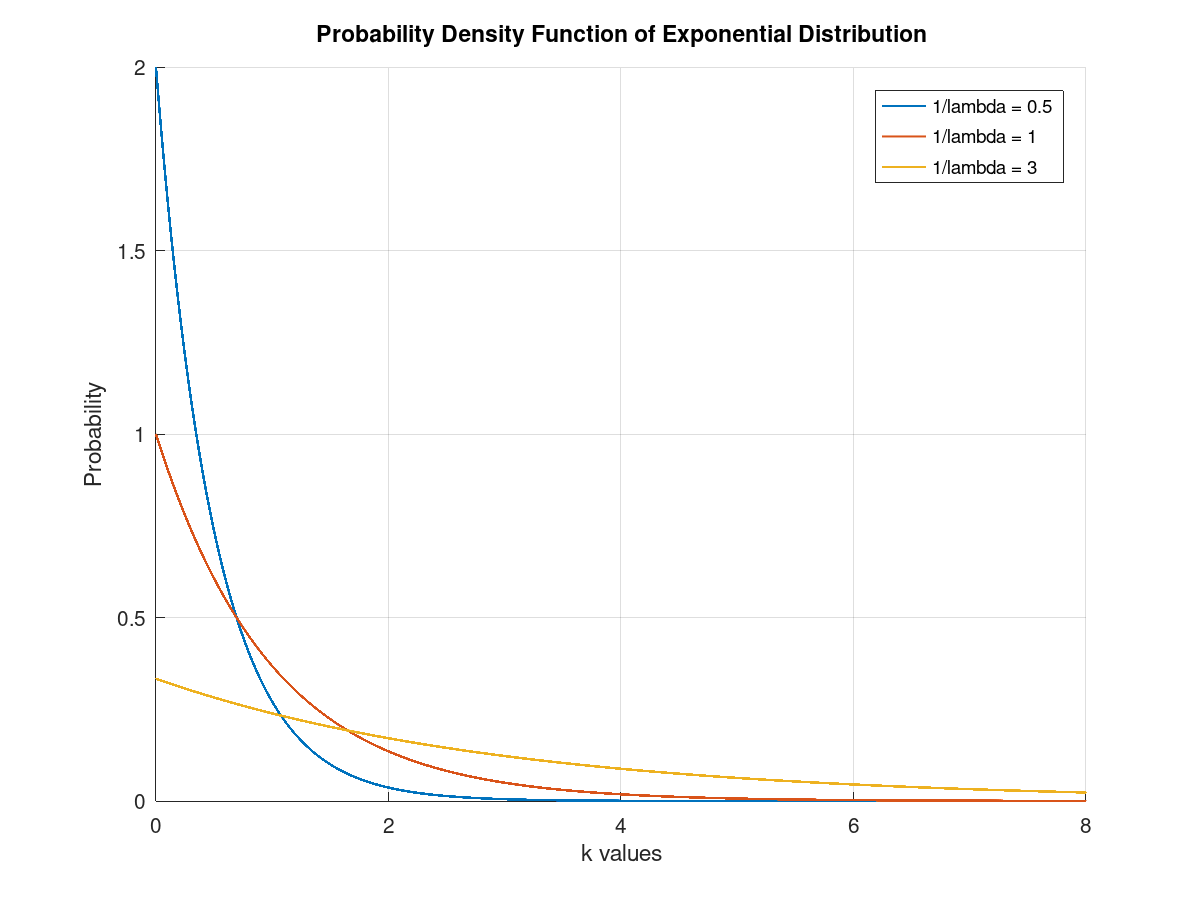
\includegraphics[width=\textwidth]{../images/Exponential_Distribution_A.png}
	\caption{Probability Density Function of Exponential Distribution}
	\label{fig:Exponential Distribution A}
\end{figure}

\subsection*{Β.}

Αντίστοιχα, με τον ίδιο τρόπο απεικονίζουμε την αθροιστική συνάρτηση κατανομής, πάλι για $ \frac{1}{λ} = \{0.5,1,3\}$:

\begin{figure}[H]
	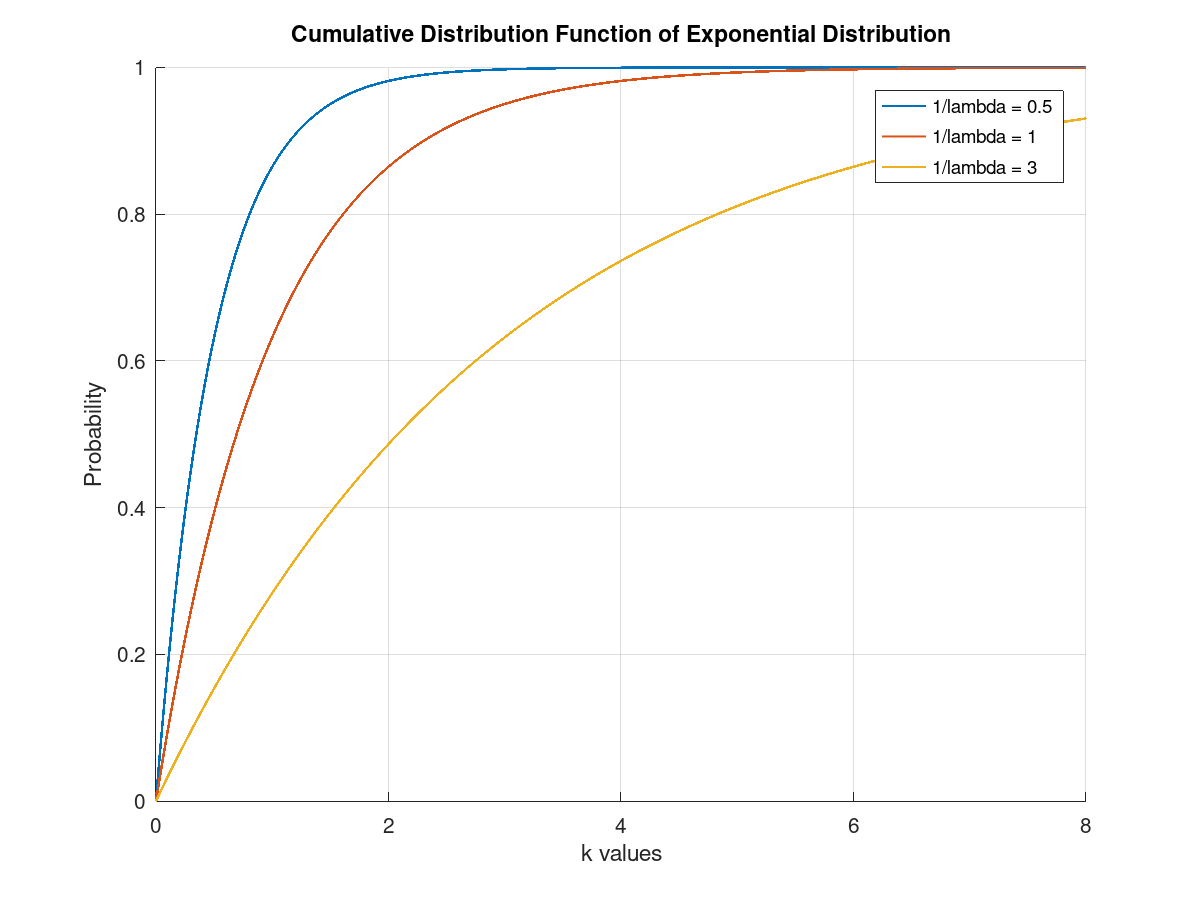
\includegraphics[width=\textwidth]{../images/Exponential_Distribution_B.png}
	\caption{Cumulative Distribution Function of Exponential Distribution}
	\label{fig:Exponential Distribution B}
\end{figure}

\subsection*{Γ.}

Χρησιμοποιώντας την συνάρτηση \textbf{exppdf()} και τον ορισμό της δεσμευμένης πιθανότητας, υπολογίζουμε τις ζητούμενες τιμές:

\lstinputlisting{../images/Exponential_Distribution_C.txt}

Παρατηρούμε ότι οι δύο πιθανότητες είναι ίσες. 
Για να δούμε γιατί ισχύει αυτή η ισότητα, υπολογίζουμε λίγο πιο αναλυτικά τις πιθανότητες και έχουμε: 
\begin{align*}
	P(X>k[50000]|X>k[20000]) &= \frac{P(X>k[50000] \cap X>k[20000])}{P(X>k[20000])} \\
							 &= \frac{P(X>k[50000])}{P(X>k[20000])} \\
							 &= \frac{e^{λ \cdot k[50000]}}{e^{λ \cdot k[20000]}} \\
							 &= e^{λ \cdot k[30000]} \\
							 &= P(X>k [30000])
\end{align*}

Στην ουσία αποδείξαμε μία ειδική περίπτωση της ιδιότητας απώλειας μνήμης, χαρακτηριστικής ιδιότητας της εκθετικής κατανομής. Η ιδιότητα αυτή υπαγορεύει ότι:
\[
	P[X>t+s|X>s] = P[X>t]
\]
Μία πιο πρακτική ερμηνεία αυτής της ιδιότητας είναι ότι, αν ο χρόνος αναμονής κάποιας διαδικασίας μοντελοποιηθεί ως εκθετική τυχαία μεταβλητή, τότε ο υπολειπόμενος χρόνος θα έχει συνεχώς την ίδια εκθετική κατανομή, χωρίς να έχει σημασία το πόσος χρόνος έχει περάσει ήδη.

\section*{Διαδικασία Καταμέτρησης Poisson}

\subsection*{Α.}

Γνωρίζουμε ότι οι χρόνοι που μεσολαβούν ανάμεσα στην εμφάνιση δύο διαδοχικών γεγονότων της διαδικασίας Poisson με παράμετρο $ λ $ ακολουθούν εκθετική κατανομή με μέση τιμή $ \frac{1}{λ} $.

Έτσι, με την εντολή \textbf{exprnd()} $ (λ = 5) $ δημιουργούμε 100 τέτοιους χρόνους, δηλαδή 100 διαδοχικά τυχαία γεγονότα, και μέσω της συνάρτησης stairs() απεικονίζουμε μία διαδικασία καταμέτρησης Poisson:

\begin{figure}[H]
	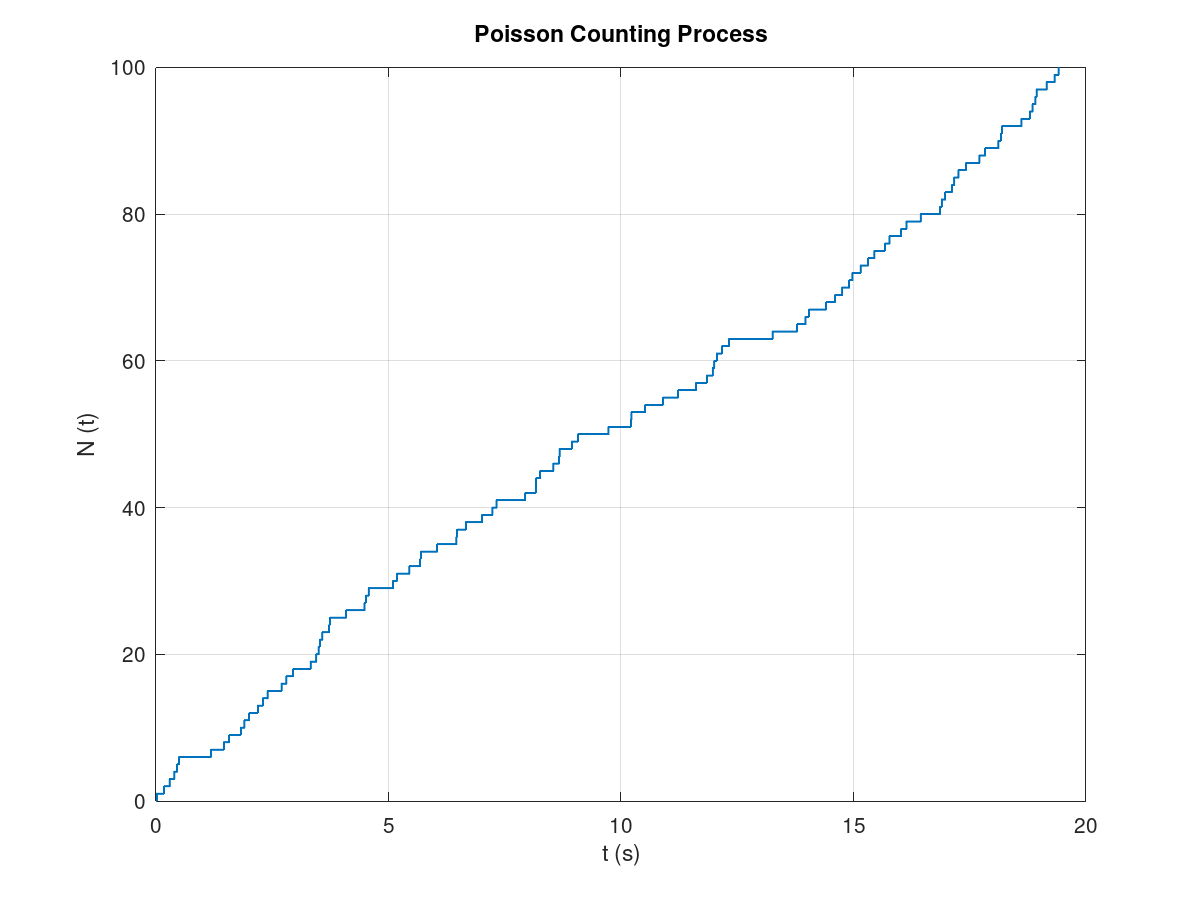
\includegraphics[width=\textwidth]{../images/Poisson_Counting_A.png}
	\caption{Poisson Counting Process}
	\label{fig:Poisson Counting A}
\end{figure}

\subsection*{Β.}

Γνωρίζουμε ότι ο αριθμός γεγονότων σε ένα χρονικό παράθυρο ${ΔΤ = t_1 - t_2 }$ ακολουθεί κατανομή Poisson με παράμετρο $ λΔΤ $  (όπου λ η παράμετρος της διαδικασίας καταμέτρησης Poisson), δηλαδή ο μέσος αριθμός εμφανίσεων είναι ανάλογος του διαστήματος $ΔΤ$.

Βρίσκουμε τον μέσο αριθμό γεγονότων στην μονάδα του χρόνου $\left(\frac{\text{ αριθμός γεγονότων}}{\text{συνολικός χρόνος}}\right)$, για $ \{200,300,500,1000,10000,100000,1000000\}$ διαδοχικά γεγονότα. Προκύπτει:

\lstinputlisting{../images/Poisson_Counting_B.txt}

Παρατηρούμε ότι όσο ο αριθμός γεγονότων μεγαλώνει, τόσο ο μέσος αριθμός γεγονότων πλησιάζει την παράμετρο $ λ = 5 \ \frac{\text{γεγονότα}}{\text{sec}} $, ως οφείλει, αφού πρόκειται για διαδικασία καταμέτρησης Poisson.

\section*{Παράρτημα Κώδικα}

\subsection*{Κατανομή Poisson}
\lstinputlisting[language=Octave]{../submission_code/Poisson_Distribution.m}


\subsection*{Εκθετική Κατανομή}
\lstinputlisting[language=Octave]{../submission_code/Exponential_Distribution.m}


\subsection*{Διαδικασία Καταμέτρησης Poisson}
\lstinputlisting[language=Octave]{../submission_code/Poisson_Counting.m}
\end{document}
